\columnratio{0.55}
\begin{paracol}{2}
 
\switchcolumn[0]*%%%%%%%
\section{State Management}
\switchcolumn
\section{状态管理}
\switchcolumn[0]*%%%%%%%
\subsection{What is State Management?}
\switchcolumn
\subsection{什么是状态管理?}
\switchcolumn[0]*%%%%%%%
Technically, every Vue component instance already "manages" its own
reactive state. Take a simple counter component as an example:
\switchcolumn
理论上来说,每一个 Vue
组件实例都已经在``管理''它自己的响应式状态了。我们以一个简单的计数器组件为例:
\switchcolumn[0]*%%%%%%%
\begin{codeHtml}
<script setup>
import { ref } from 'vue'
// 状态
const count = ref(0)
// 动作
function increment() {
  count.value++
}
</script>
<!-- 视图 -->
<template>{{ count }}</template>
\end{codeHtml}
\switchcolumn
\begin{codeHtml}
<script setup>
import { ref } from 'vue'
// 状态
const count = ref(0)
// 动作
function increment() {
  count.value++
}
</script>
<!-- 视图 -->
<template>{{ count }}</template>
\end{codeHtml}
\switchcolumn[0]*%%%%%%%
It is a self-contained unit with the following parts:
\switchcolumn
它是一个独立的单元,由以下几个部分组成:
\switchcolumn[0]*%%%%%%%
\begin{itemize}
\item
  The \textbf{state}, the source of truth that drives our app;
\item
  The \textbf{view}, a declarative mapping of the \textbf{state};
\item
  The \textbf{actions}, the possible ways the state could change in
  reaction to user inputs from the \textbf{view}.
\end{itemize}
\switchcolumn
\begin{itemize}
\item
  \textbf{状态}:驱动整个应用的数据源;
\item
  \textbf{视图}:对\textbf{状态}的一种声明式映射;
\item
  \textbf{交互}:状态根据用户在\textbf{视图}中的输入而作出相应变更的可能方式。
\end{itemize}
\switchcolumn[0]*%%%%%%%
This is a simple representation of the concept of "one-way data flow":
\switchcolumn
下面是``单向数据流''这一概念的简单图示:
\end{paracol}

\begin{center} 
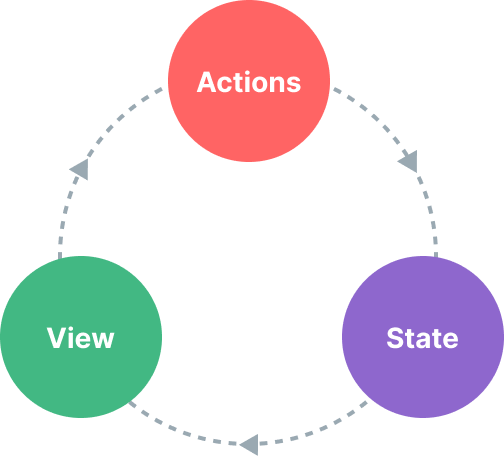
\includegraphics{./img/state-flow.a8bc738e.png} 
\end{center}
    

\columnratio{0.55}
\begin{paracol}{2}
 
\switchcolumn[0]*%%%%%%%
However, the simplicity starts to break down when we have
\textbf{multiple components that share a common state}:
\switchcolumn
然而,当我们有\textbf{多个组件共享一个共同的状态}时,就没有这么简单了:
\switchcolumn[0]*%%%%%%%
\begin{enumerate}
\item
  Multiple views may depend on the same piece of state.
\item
  Actions from different views may need to mutate the same piece of
  state.
\end{enumerate}
\switchcolumn
\begin{enumerate}
\item
  多个视图可能都依赖于同一份状态。
\item
  来自不同视图的交互也可能需要更改同一份状态。
\end{enumerate}
\switchcolumn[0]*%%%%%%%
For case one, a possible workaround is by "lifting" the shared state up
to a common ancestor component, and then pass it down as props. However,
this quickly gets tedious in component trees with deep hierarchies,
leading to another problem known as
\href{https://vuejs.org/guide/components/provide-inject.html\#prop-drilling}{Prop
Drilling}.
\switchcolumn
对于情景
1,一个可行的办法是将共享状态``提升''到共同的祖先组件上去,再通过 props
传递下来。然而在深层次的组件树结构中这么做的话,很快就会使得代码变得繁琐冗长。这会导致另一个问题:\href{https://cn.vuejs.org/guide/components/provide-inject.html\#prop-drilling}{Prop
逐级透传问题}。
\switchcolumn[0]*%%%%%%%
For case two, we often find ourselves resorting to solutions such as
reaching for direct parent / child instances via template refs, or
trying to mutate and synchronize multiple copies of the state via
emitted events. Both of these patterns are brittle and quickly lead to
unmaintainable code.
\switchcolumn
对于情景
2,我们经常发现自己会直接通过模板引用获取父/子实例,或者通过触发的事件尝试改变和同步多个状态的副本。但这些模式的健壮性都不甚理想,很容易就会导致代码难以维护。
\switchcolumn[0]*%%%%%%%
A simpler and more straightforward solution is to extract the shared
state out of the components, and manage it in a global singleton. With
this, our component tree becomes a big "view", and any component can
access the state or trigger actions, no matter where they are in the
tree!
\switchcolumn
一个更简单直接的解决方案是抽取出组件间的共享状态,放在一个全局单例中来管理。这样我们的组件树就变成了一个大的``视图'',而任何位置上的组件都可以访问其中的状态或触发动作。
\switchcolumn[0]*%%%%%%%
\subsection{Simple State Management with Reactivity API}
\switchcolumn
\subsection{用响应式 API 做简单状态管理}
\switchcolumn[0]*%%%%%%%
If you have a piece of state that should be shared by multiple
instances, you can use
\href{https://vuejs.org/api/reactivity-core.html\#reactive}{\texttt{reactive()}}
to create a reactive object, and then import it into multiple
components:
\switchcolumn
如果你有一部分状态需要在多个组件实例间共享,你可以使用
\href{https://cn.vuejs.org/api/reactivity-core.html\#reactive}{\texttt{reactive()}}
来创建一个响应式对象,并将它导入到多个组件中:
\switchcolumn[0]*%%%%%%%
\begin{codeJs}
// store.js
import { reactive } from 'vue'
export const store = reactive({
  count: 0
})
\end{codeJs}
\switchcolumn
\begin{codeJs}
// store.js
import { reactive } from 'vue'
export const store = reactive({
  count: 0
})
\end{codeJs}
\switchcolumn[0]*%%%%%%%
\begin{codeHtml}
<!-- ComponentA.vue -->
<script setup>
import { store } from './store.js'
</script>
<template>From A: {{ store.count }}</template>
\end{codeHtml}
\switchcolumn
\begin{codeHtml}
<!-- ComponentA.vue -->
<script setup>
import { store } from './store.js'
</script>
<template>From A: {{ store.count }}</template>
\end{codeHtml}
\switchcolumn[0]*%%%%%%%
\begin{codeHtml}
<!-- ComponentB.vue -->
<script setup>
import { store } from './store.js'
</script>
<template>From B: {{ store.count }}</template>
\end{codeHtml}
\switchcolumn
\begin{codeHtml}
<!-- ComponentB.vue -->
<script setup>
import { store } from './store.js'
</script>
<template>From B: {{ store.count }}</template>
\end{codeHtml}
\switchcolumn[0]*%%%%%%%
Now whenever the \texttt{store} object is mutated, both
\texttt{\textless{}ComponentA\textgreater{}} and
\texttt{\textless{}ComponentB\textgreater{}} will update their views
automatically - we have a single source of truth now.
\switchcolumn
现在每当 \texttt{store}
对象被更改时,\texttt{\textless{}ComponentA\textgreater{}} 与
\texttt{\textless{}ComponentB\textgreater{}}
都会自动更新它们的视图。现在我们有了单一的数据源。
\switchcolumn[0]*%%%%%%%
However, this also means any component importing \texttt{store} can
mutate it however they want:
\switchcolumn
然而,这也意味着任意一个导入了 \texttt{store}
的组件都可以随意修改它的状态:
\switchcolumn[0]*%%%%%%%
\begin{codeHtml}
<template>
  <button @click="store.count++">
    From B: {{ store.count }}
  </button>
</template>
\end{codeHtml}
\switchcolumn
\begin{codeHtml}
<template>
  <button @click="store.count++">
    From B: {{ store.count }}
  </button>
</template>
\end{codeHtml}
\switchcolumn[0]*%%%%%%%
While this works in simple cases, global state that can be arbitrarily
mutated by any component is not going to be very maintainable in the
long run. To ensure the state-mutating logic is centralized like the
state itself, it is recommended to define methods on the store with
names that express the intention of the actions:
\switchcolumn
虽然这在简单的情况下是可行的,但从长远来看,可以被任何组件任意改变的全局状态是不太容易维护的。为了确保改变状态的逻辑像状态本身一样集中,建议在
store 上定义方法,方法的名称应该要能表达出行动的意图:
\switchcolumn[0]*%%%%%%%
\begin{codeJs}
// store.js
import { reactive } from 'vue'
export const store = reactive({
  count: 0,
  increment() {
    this.count++
  }
})
\end{codeJs}
\switchcolumn
\begin{codeJs}
// store.js
import { reactive } from 'vue'
export const store = reactive({
  count: 0,
  increment() {
    this.count++
  }
})
\end{codeJs}
\switchcolumn[0]*%%%%%%%
\begin{codeHtml}
<template>
  <button @click="store.increment()">
    From B: {{ store.count }}
  </button>
</template>
\end{codeHtml}
\switchcolumn
\begin{codeHtml}
<template>
  <button @click="store.increment()">
    From B: {{ store.count }}
  </button>
</template>
\end{codeHtml}
\switchcolumn[0]*%%%%%%%
\href{https://play.vuejs.org/\#eNrNkk1uwyAQha8yYpNEiUzXllPVrtRTeJNSqtLGgGBsVbK4ewdwnT9FWWSTFczwmPc+xMhqa4uhl6xklRdOWQQvsbfPrVadNQ7h1dCqpcYaPp3pYFHwQyteXVxKm0tpM0krnm3IgAqUnd3vUFIFUB1Z8bNOkzoVny+wDTuNcZ1gBI/GSQhzqlQX3/5Gng81pA1t33tEo+FF7JX42bYsT1BaONlRguWqZZMU4C261CWMk3EhTK8RQphm8Twse/BscoUsvdqDkTX3kP3nI6aZwcmdQDUcMPJPabX8TQphtCf0RLqd1csxuqQAJTxtYnEUGtIpAH4pn1Ou17FDScOKhT+QNAVM}{Try
it in the Playground}
\switchcolumn
\href{https://play.vuejs.org/\#eNrNkk1uwyAQha8yYpNEiUzXllPVrtRTeJNSqtLGgGBsVbK4ewdwnT9FWWSTFczwmPc+xMhqa4uhl6xklRdOWQQvsbfPrVadNQ7h1dCqpcYaPp3pYFHwQyteXVxKm0tpM0krnm3IgAqUnd3vUFIFUB1Z8bNOkzoVny+wDTuNcZ1gBI/GSQhzqlQX3/5Gng81pA1t33tEo+FF7JX42bYsT1BaONlRguWqZZMU4C261CWMk3EhTK8RQphm8Twse/BscoUsvdqDkTX3kP3nI6aZwcmdQDUcMPJPabX8TQphtCf0RLqd1csxuqQAJTxtYnEUGtIpAH4pn1Ou17FDScOKhT+QNAVM}{在演练场中尝试一下}
\switchcolumn[0]*%%%%%%%
\begin{vueQuote}{TIP}
Note the click handler uses \texttt{store.increment()} with parentheses
- this is necessary to call the method with the proper \texttt{this}
context since it's not a component method.
\end{vueQuote} 
\switchcolumn
\begin{vueQuote}{TIP}
请注意这里点击的处理函数使用了
\texttt{store.increment()},带上了圆括号作为内联表达式调用,因为它并不是组件的方法,并且必须要以正确的
\texttt{this} 上下文来调用。
\end{vueQuote} 
\switchcolumn[0]*%%%%%%%
Although here we are using a single reactive object as a store, you can
also share reactive state created using other
\href{https://vuejs.org/api/reactivity-core.html}{Reactivity APIs} such
as \texttt{ref()} or \texttt{computed()}, or even return global state
from a
\href{https://vuejs.org/guide/reusability/composables.html}{Composable}:
\switchcolumn
除了我们这里用到的单个响应式对象作为一个 store
之外,你还可以使用其他\href{https://cn.vuejs.org/api/reactivity-core.html}{响应式
API} 例如 \texttt{ref()} 或是
\texttt{computed()},或是甚至通过一个\href{https://cn.vuejs.org/guide/reusability/composables.html}{组合式函数}来返回一个全局状态:
\switchcolumn[0]*%%%%%%%
\begin{codeJs}
import { ref } from 'vue'
// 全局状态,创建在模块作用域下
const globalCount = ref(1)
export function useCount() {
  // 局部状态,每个组件都会创建
  const localCount = ref(1)
  return {
    globalCount,
    localCount
  }
}
\end{codeJs}
\switchcolumn
\begin{codeJs}
import { ref } from 'vue'
// 全局状态,创建在模块作用域下
const globalCount = ref(1)
export function useCount() {
  // 局部状态,每个组件都会创建
  const localCount = ref(1)
  return {
    globalCount,
    localCount
  }
}
\end{codeJs}
\switchcolumn[0]*%%%%%%%
The fact that Vue's reactivity system is decoupled from the component
model makes it extremely flexible.
\switchcolumn
事实上,Vue 的响应性系统与组件层是解耦的,这使得它非常灵活。
\end{paracol}

\columnratio{0.55}
\begin{paracol}{2}
 
\switchcolumn[0]*%%%%%%%
\subsection{SSR Considerations}
\switchcolumn
\subsection{SSR 相关细节}
\switchcolumn[0]*%%%%%%%
If you are building an application that leverages
\href{https://vuejs.org/guide/scaling-up/ssr.html}{Server-Side Rendering
(SSR)}, the above pattern can lead to issues due to the store being a
singleton shared across multiple requests. This is discussed in
\href{https://vuejs.org/guide/scaling-up/ssr.html\#cross-request-state-pollution}{more
details} in the SSR guide.
\switchcolumn
如果你正在构建一个需要利用\href{https://cn.vuejs.org/guide/scaling-up/ssr.html}{服务端渲染
(SSR)} 的应用,由于 store
是跨多个请求共享的单例,上述模式可能会导致问题。这在 SSR
指引那一章节会讨论\href{https://cn.vuejs.org/guide/scaling-up/ssr.html\#cross-request-state-pollution}{更多细节}。
\switchcolumn[0]*%%%%%%%
\subsection{Pinia}
\switchcolumn
\subsection{Pinia}
\switchcolumn[0]*%%%%%%%
While our hand-rolled state management solution will suffice in simple
scenarios, there are many more things to consider in large-scale
production applications:
\switchcolumn
虽然我们的手动状态管理解决方案在简单的场景中已经足够了,但是在大规模的生产应用中还有很多其他事项需要考虑:
\switchcolumn[0]*%%%%%%%
\begin{itemize}
\item
  Stronger conventions for team collaboration
\item
  Integrating with the Vue DevTools, including timeline, in-component
  inspection, and time-travel debugging
\item
  Hot Module Replacement
\item
  Server-Side Rendering support
\end{itemize}
\switchcolumn
\begin{itemize}
\item
  更强的团队协作约定
\item
  与 Vue DevTools 集成,包括时间轴、组件内部审查和时间旅行调试
\item
  模块热更新 (HMR)
\item
  服务端渲染支持
\end{itemize}
\switchcolumn[0]*%%%%%%%
\href{https://pinia.vuejs.org/}{Pinia} is a state management library
that implements all of the above. It is maintained by the Vue core team,
and works with both Vue 2 and Vue 3.
\switchcolumn
\href{https://pinia.vuejs.org/zh/}{Pinia}
就是一个实现了上述需求的状态管理库,由 Vue 核心团队维护,对 Vue 2 和 Vue
3 都可用。
\switchcolumn[0]*%%%%%%%
Existing users may be familiar with
\href{https://vuex.vuejs.org/}{Vuex}, the previous official state
management library for Vue. With Pinia serving the same role in the
ecosystem, Vuex is now in maintenance mode. It still works, but will no
longer receive new features. It is recommended to use Pinia for new
applications.
\switchcolumn
现有用户可能对 \href{https://vuex.vuejs.org/zh/}{Vuex} 更熟悉,它是 Vue
之前的官方状态管理库。由于 Pinia
在生态系统中能够承担相同的职责且能做得更好,因此 Vuex
现在处于维护模式。它仍然可以工作,但不再接受新的功能。对于新的应用,建议使用
Pinia。
\switchcolumn[0]*%%%%%%%
Pinia started out as an exploration of what the next iteration of Vuex
could look like, incorporating many ideas from core team discussions for
Vuex 5. Eventually, we realized that Pinia already implements most of
what we wanted in Vuex 5, and decided to make it the new recommendation
instead.
\switchcolumn
事实上,Pinia 最初正是为了探索 Vuex
的下一个版本而开发的,因此整合了核心团队关于 Vuex 5
的许多想法。最终,我们意识到 Pinia 已经实现了我们想要在 Vuex 5
中提供的大部分内容,因此决定将其作为新的官方推荐。
\switchcolumn[0]*%%%%%%%
Compared to Vuex, Pinia provides a simpler API with less ceremony,
offers Composition-API-style APIs, and most importantly, has solid type
inference support when used with TypeScript.
\switchcolumn
相比于 Vuex,Pinia 提供了更简洁直接的 API,并提供了组合式风格的
API,最重要的是,在使用 TypeScript 时它提供了更完善的类型推导。
\end{paracol}

